\setlength{\parindent}{0pt}
\chapter{Casualties} \label{chap:casualties}

Currently, a large part of the world is contaminated by mines and ERW as seen in figure \textbf{\ref{fig:contamination_mine_erw}}, this affects a large number of people in their day to day life. Landmines do not discriminate. Thus victims can be men, women, children, people from all nationalities, and ages. Hence as mentioned in the introduction, the Anti-Personnel Mine Ban Treaty was introduced in 1999, which has lead to yearly rising contributions from the state parties ever since. \cite{LandmineMonitor2019} 

        \vspace{5mm}

\begin{centering}

\textit{\large “A landmine is the perfect soldier: Ever courageous, never sleeps, never misses"}\\

\begin{flushright}

        \vspace{-3mm}
        
-- Paul Jefferson, one of the earliest humanitarian deminers \hspace{4mm}

\end{flushright}
\end{centering}

%%%

\section{Casualties in Numbers}

% First use: \gls{svm}. Second use: \gls{svm}.

The landmine monitor 2019 is a report formed by the \gls{icbl} and the \gls{cmc}, the data in the report is processed by the Monitoring and Research Committee, a standing committee of the ICBL-CMC Governance Board. Which is comprised of five \gls{ngo}s, as well as Monitor research team leaders and ICBL-CMC staff and contributions from 11 countries. All of them contributing to writing the annual landmine monitoring report. Furthermore, the landmine monitor is approved and provided by the \gls{un} \cite{LandmineMonitor2019}.

        \vspace{2mm}

\begin{figure}[h]
  \centering
  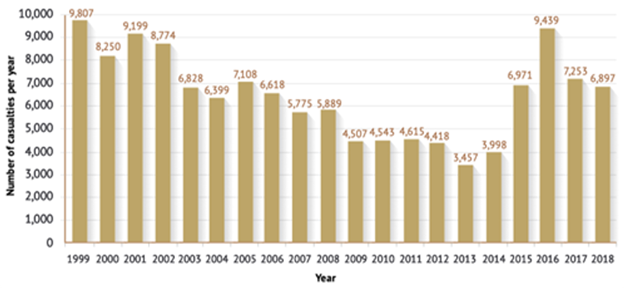
\includegraphics[width=12.5cm]{00 - Images/casualties_per_year.png}
  \caption{Casualties annually due to landmines/\gls{erw} (1999-2018) \cite{LandmineMonitor2019}}
  \label{fig:casualties_per_year}
\end{figure}

\newpage

An increase in conflicts and wars in 2014-16, entails a big spike in the global number of casualties by landmines, as seen in Figure \ref{fig:casualties_per_year}. These casualties come from two main categories of explosive war remains: The standard landmines and the \gls{erw}, which covers the \gls{uxo}. UXOs include weapons that failed to detonate and \gls{axo}. AXOs are weapons that have never been used in conflicts and were abandoned by the party that owned it \cite{Remnants2019:online}. 

        \vspace{2mm}

As a result of the Mine Ban Treaty, the people who still use these banned explosives turned to make homemade and improvised mines, which is why most mines are of this kind today. This causes a lot of problems, because of the variety in design and internal contents of the mines, which makes it difficult to remove and destroy them. This is due to a lack of knowledge of the construction of the mines. The lack of reporting to the authorities, when an improvised mine is planted, entails many unrecorded casualties. In 2009-2014 where the global landmine casualties were at its lowest, it was estimated that there was annually between 700 and 1300 extra casualties, which is not included in these statistics. 

        \vspace{2mm}

Since the mine ban treaty was initially introduced, back in 1999, there have been recorded 130.745 casualties. The total sum of casualties in different countries is still rising every day, the 2019 report states that; the estimated number of casualties per day worldwide is 18 during the 19-year period from 1999-2018 \cite{LandmineMonitor2019}.

        \vspace{2mm}

\begin{wrapfigure}[15]{r}{0.50\textwidth}
    \vspace{-5mm}
    \centering
      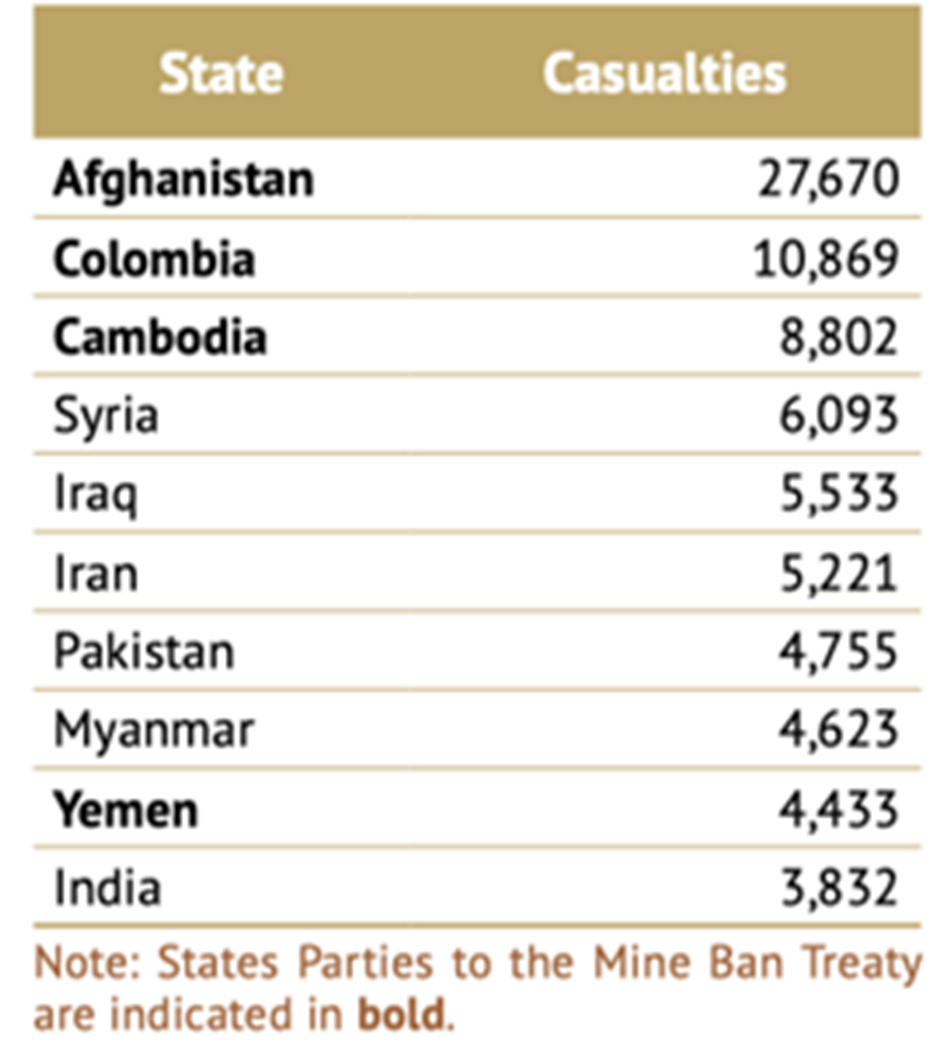
\includegraphics[width=0.45\textwidth]{00 - Images/casualties_per_country.png}
  \caption{Countries with the highest total casualties (1999 – 2018) \cite{LandmineMonitor2019}}
  \label{fig:casualties_per_country}
\end{wrapfigure}

Figure \ref{fig:casualties_per_country} states the countries with the highest total casualties from 1999-2018 caused by mines/\gls{erw}, were countries such as Afghanistan, Colombia, and Cambodia had a death count of 47.341 people - this corresponds to 36,2\% of the total casualties during this period. These countries are or were experiencing conflicts and are members of the mine ban treaty, which implies that these countries have a higher number of improvised mines. This results in increased difficulty in removing the landmines. Furthermore, the listed countries have very different environments that raise yet another problem, and a need for a problem limitation, or a universal solution which can locate mines in all kinds of terrain \cite{LandmineMonitor2019}.

\clearpage

\section{Casualty Demographics}
Statistics show that there were at least 1.714 child\footnote{Child casualties are defined as all casualties where the victim is less than 18 years of age at the time of the incident.} casualties in 2018 caused by mines/\gls{erw}. The child casualties made up 40\% of all the casualties where the age was known. The statistics distinguish the sex of the children, showing that the vast majority corresponding to 84\% are boys.

        \vspace{2mm}

A broad look at the statistics from 2018 men and boys made up 88\% of the casualties, whereas women and girls made up the remaining 12\% of all casualties where the sex was known. Civilians represented 71\% of casualties where the status\footnote{The status ranges between military, civilian, deminer} was known - these casualties were recorded in 38 states in different areas \cite{LandmineMonitor2019}.

\section{Casualties by Mine Type}

In 2018, mines caused at least 4.885 casualties in total. These can be split up into four groups: 
\begin{itemize}
    \item Antipersonnel mines
            \vspace{-4mm}
    \item Anti-vehicle mines
            \vspace{-4mm}
    \item Improvised mines
            \vspace{-4mm}
    \item Other unspecified mines
\end{itemize}

The deadliest type of mine is the improvised mine, causing 3.789 casualties, which is the largest part of the total casualties registered, as seen in Figure \ref{fig:casualties_by_type}. Out of the 3.789 casualties, it was recorded that 1.752 (46\%) of these casualties were identified to be specifically improvised, antipersonnel mines. \gls{erw} does also have a large place in the statistics, causing 1.410 casualties \cite{LandmineMonitor2019}.

\begin{figure}[h]
  \centering
  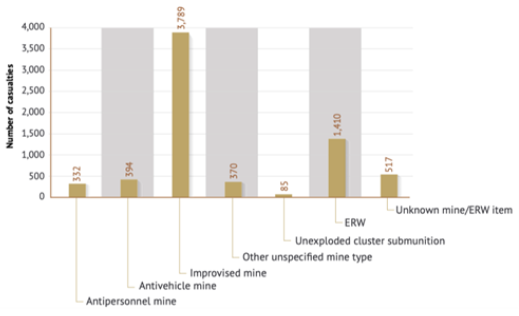
\includegraphics[width=12.5cm]{00 - Images/casualties_by_type.png}
  \caption{Casualties by type of mine/\gls{erw} in 2018 \cite{LandmineMonitor2019}}
  \label{fig:casualties_by_type}
\end{figure}